\documentclass{math}

\usepackage{pgfplots}
\pgfplotsset{compat=1.13}

\geometry{letterpaper, margin=0.5in}

\title{Differential Equations: Homework 1}
\author{Alvin Lin}
\date{January 2018 - May 2018}

\begin{document}

\maketitle
\clearpage

\subsection*{Exercise 1}
Show that \( \phi(x) = x^2 \) is an explicit solution to
\[ x\ddiff{y}{x} = 2y \]
on the interval \( (-\infty,\infty) \).
\begin{align*}
  \phi(x) &= x^2 \\
  \phi'(x) &= 2x \\
  x\ddiff{y}{x} &= 2y \\
  x(2x) &= 2(x^2) \\
  2x^2 &= 2x^2
\end{align*}
Show that \( \phi(x) = \e^x-x \) is an explicit solution to
\[ \ddiff{y}{x}+y^2 = \e^{2x}+(1-2x)\e^x+x^2-1 \]
on the interval \( (-\infty,\infty) \).
\begin{align*}
  \phi(x) &= \e^x-x \\
  \phi'(x) &= \e^x-1 \\
  \ddiff{y}{x}+y^2 &= \e^{2x}+(1-2x)\e^x+x^2-1 \\
  \e^x-1+(\e^x-x)^2 &= \e^{2x}+(1-2x)\e^x+x^2-1 \\
  \e^x-1+(\e^{2x}-2x\e^x+x^2) &= \e^{2x}+(1-2x)\e^x+x^2-1 \\
  \e^{2x}+\e^x-2x\e^x+x^2-1 &= \e^{2x}+(1-2x)\e^x+x^2-1 \\
  \e^{2x}+(1-2x)\e^x+x^2-1 &= \e^{2x}+(1-2x)\e^x+x^2-1
\end{align*}
Show that \( \phi(x) = x^2-x^{-1} \) is an explicit solution to
\[ x^2\ddiff{^2y}{x^2} = 2y \]
on the interval \( (0,\infty) \).
\begin{align*}
  \phi(x) &= x^2-\frac{1}{x} \\
  \phi'(x) &= 2x+x^{-2} \\
  \phi''(x) &= 2-\frac{2}{x^3} \\
  x^2\ddiff{^2y}{x^2} &= 2y \\
  x^2(2-\frac{2}{x^3}) &= 2(x^2-\frac{1}{x}) \\
  2x^2-\frac{2}{x} &= 2x^2-\frac{2}{x}
\end{align*}

\subsection*{Exercise 2}
Show that \( y^2+x-3 = 0 \) is an implicit solution to \( \ddiff{y}{x} =
\frac{-1}{2y} \) on the interval \( (-\infty,3) \).
\begin{align*}
  y^2+x-3 &= 0 \\
  2y\ddiff{y}{x}+1 &= 0 \\
  2y\ddiff{y}{x} &= -1 \\
  \ddiff{y}{x} &= \frac{-1}{2y}
\end{align*}
Show that \( xy^3-xy^3\sin(x) = 1 \) is an implicit solution to
\[ \ddiff{y}{x} = \frac{(x\cos(x)+\sin(x)-1)y}{3(x-x\sin(x))} \]
on the interval \( (0,\frac{\pi}{2}) \).
\begin{align*}
  xy^3-xy^3\sin(x) &= 1 \\
  \ddiff{}{x}(xy^3)-
    \left[\ddiff{}{x}(xy^3)\sin(x)+xy^3\ddiff{}{x}(\sin(x))\right] &= 0 \\
  (1-\sin(x))\ddiff{}{x}(xy^3)-xy^3\cos(x) &= 0 \\
  (1-\sin(x))(3xy^2\ddiff{y}{x}+y^3)-xy^3\cos(x) &= 0 \\
  3xy^2\ddiff{y}{x}+y^3-3xy^2\sin(x)\ddiff{y}{x}-y^3\sin(x)-xy^3\cos(x) &= 0 \\
  3xy^2\ddiff{y}{x}-3xy^2\sin(x)\ddiff{y}{x} &= xy^3\cos(x)+y^3\sin(x)-y^3 \\
  \ddiff{y}{x}3y^2(x-x\sin(x)) &= (x\cos(x)+\sin(x)-1)y^3 \\
  \ddiff{y}{x} &= \frac{(x\cos(x)+\sin(x)-1)y^3}{3y^2(x-x\sin(x))} \\
  \ddiff{y}{x} &= \frac{(x\cos(x)+\sin(x)-1)y}{3(x-x\sin(x))} \\
\end{align*}

\subsection*{Exercise 3}
Determine whether the given function is a solution to the given differential
equation.
\[ y = \sin(x)+x^2 \quad \ddiff{^2y}{x^2}+y = x^2+2 \]
\begin{align*}
  y &= \sin(x)+x^2 \\
  \ddiff{y}{x} &= \cos(x)+2x \\
  \ddiff{^2y}{x^2} &= -\sin(x)+2 \\
  \ddiff{^2y}{x^2}+y &= x^2+2 \\
  (-\sin(x)+2)+(\sin(x)+x^2) &= x^2+2 \\
  x^2+2 &= x^2+2
\end{align*}

\subsection*{Exercise 6}
Determine whether the given function is a solution to the given differential
equation.
\[ x = \cos(t) \quad \ddiff{x}{t}+tx = \sin(2t) \]
\begin{align*}
  x &= \cos(2t) \\
  \ddiff{x}{t} &= -2\sin(2t) \\
  \ddiff{x}{t}+tx &= \sin(2t) \\
  -2\sin(2t)+t(\cos(2t)) &= \sin(2t) \\
  t\cos(2t) &= 3\sin(2t) \\
\end{align*}
No solution.

\subsection*{Exercise 7}
Determine whether the given function is a solution to the given differential
equation.
\[ y = \e^{2x}-3\e^{-x} \quad \ddiff{^2y}{x^2}-\ddiff{y}{x}-2y = 0 \]
\begin{align*}
  y &= \e^{2x}-3\e^{-x} \\
  \ddiff{y}{x} &= 2\e^{2x}+3\e^{-x} \\
  \ddiff{^2y}{x^2} &= 4\e^{2x}-3\e^{-x} \\
  \ddiff{^2y}{x^2}-\ddiff{y}{x}-2y &= 0 \\
  (4\e^{2x}-3\e^{-x})-(2\e^{2x}+3\e^{-x})-2(\e^{2x}-3\e^{-x}) &= 0 \\
  0 &= 0
\end{align*}

\subsection*{Exercise 8}
Determine whether the given function is a solution to the given differential
equation.
\[ y = 3\sin(2x)+\e^{-x} \quad y''+4y = 5\e^{-x} \]
\begin{align*}
  y &= 3\sin(2x)+\e^{-x} \\
  y' &= 6\cos(2x)-\e^{-x} \\
  y'' &= -12\sin(2x)+\e^{-x} \\
  y''+4y &= 5\e^{-x} \\
  (-12\sin(2x)+\e^{-x})+4(3\sin(2x)+\e^{-x}) &= 5\e^{-x} \\
  5\e^{-x} &= 5\e^{-x}
\end{align*}

\subsection*{Exercise 9}
Determine whether the given relation is an implicit solution to the given
differential equation. Assume that the relationship does define \( y \)
implicitly as a function of \( x \) and use implicit differentiation.
\[ x^2+y^2 = 4 \quad \ddiff{y}{x} = \frac{x}{y} \]
\begin{align*}
  x^2+y^2 &= 4 \\
  2x+2y\ddiff{y}{x} &= 0 \\
  \ddiff{y}{x}2y &= -2x \\
  \ddiff{y}{x} &= \frac{-x}{y}
\end{align*}
Not a solution.

\subsection*{Exercise 10}
Determine whether the given relation is an implicit solution to the given
differential equation. Assume that the relationship does define \( y \)
implicitly as a function of \( x \) and use implicit differentiation.
\[ y-\ln(y) = x^2+1 \quad \ddiff{y}{x} = \frac{2xy}{y-1} \]
\begin{align*}
  y-\ln(y) &= x^2-1 \\
  \ddiff{y}{x}-\ddiff{y}{x}\frac{1}{y} &= 2x \\
  \ddiff{y}{x}(1-\frac{1}{y}) &= 2x \\
  \ddiff{y}{x}(y-1) &= 2xy \\
  \ddiff{y}{x} &= \frac{2xy}{y-1}
\end{align*}

\subsection*{Exercise 11}
Determine whether the given relation is an implicit solution to the given
differential equation. Assume that the relationship does define \( y \)
implicitly as a function of \( x \) and use implicit differentiation.
\[ \e^{xy}+y = x-1 \quad \ddiff{y}{x} = \frac{\e^{-xy}-y}{\e^{-xy}+x} \]
\begin{align*}
  \e^{xy}+y &= x-1 \\
  \e^{xy}\ddiff{}{x}(xy)+\ddiff{y}{x} &= 1 \\
  \e^{xy}(x\ddiff{y}{x}+y)+\ddiff{y}{x} &= 1 \\
  \ddiff{y}{x}x\e^{xy}+y\e^{xy}+\ddiff{y}{x} &= 1 \\
  \ddiff{y}{x}(1+x\e^{xy}) &= 1-y\e^{xy} \\
  \ddiff{y}{x} &= \frac{1-y\e^{xy}}{1+x\e^{xy}}
\end{align*}
Not a solution.

\subsection*{Exercise 17}
Show that \( \phi(x) = C\e^{3x}+1 \) is a solution to \( \ddiff{y}{x}-3y = -3 \)
for any choice of the constant \( C \). Thus, \( C\e^{3x}+1 \) is a
one-parameter family of solutions to the differential equation. Graph several of
the solution curves using the same coordinate axes.
\begin{align*}
  \phi(x) &= C\e^{3x}+1 \\
  \phi'(x) &= 3C\e^{3x} \\
  \ddiff{y}{x}-3y &= -3 \\
  3C\e^{3x}-3(C\e^{3x}+1) &= -3 \\
  -3 &= -3
\end{align*}
\begin{center}
  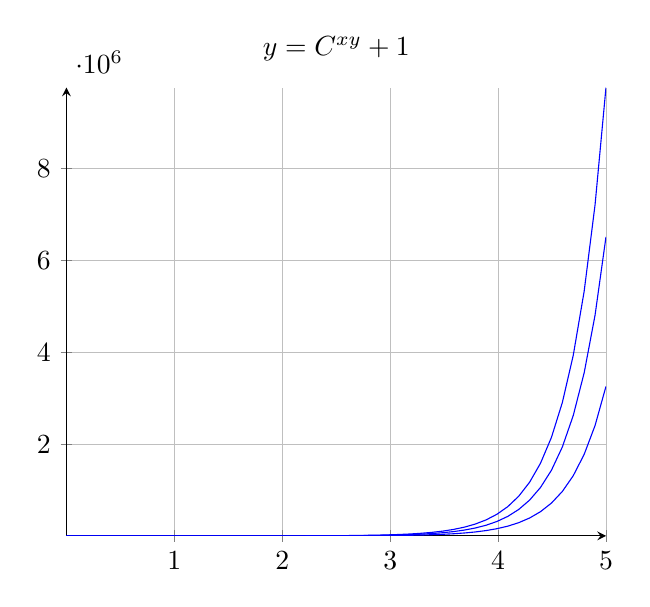
\begin{tikzpicture}
    \begin{axis}[
      title={\( y = C\e^{xy}+1 \)},
      grid=both,
      axis lines=middle,
      xmin=0, xmax=5
    ]
      \addplot[blue, samples=100] {2.7182^(3*x)+1};
      \addplot[blue, samples=100] {2*(2.7182^(3*x))+1};
      \addplot[blue, samples=100] {3*(2.7182^(3*x))+1};
    \end{axis}
  \end{tikzpicture}
\end{center}

\subsection*{Exercise 19}
Show that the equation \( (\ddiff{y}{x})^2+y^2+4 = 0 \) has no (real-valued)
solution.
\begin{align*}
  (\ddiff{y}{x})^2+y^2+4 &= 0 \\
  \ddiff{y}{x} &= \pm\sqrt{-y^2-4} \\
  \ddiff{y}{x} &= \pm\sqrt{-1}\sqrt{y^2+4} \\
  \ddiff{y}{x} &= \pm\sqrt{y^2+4}i
\end{align*}
Solutions are imaginary.

\subsection*{Exercise 22}
Verify that the function \( \phi(x) = c_1\e^x+c_2\e^{-2x} \) is a solution to
the linear equation
\[ \ddiff{^2y}{x^2}+\ddiff{y}{x}-2y = 0 \]
for any choice of the constants \( c_1 \) and \( c_2 \).
\begin{align*}
  \phi(x) &= c_1\e^x+c_2\e^{-2x} \\
  \phi'(x) &= c_1\e^x-2c_2\e^{-2x} \\
  \phi''(x) &= c_1\e^x+4c_2\e^{-2x} \\
  \ddiff{^2y}{x^2}+\ddiff{y}{x}-2y &= 0 \\
  (c_1\e^x+4c_2\e^{-2x})+(c_1\e^x-2c_2\e^{-2x})-2(c_1\e^x+c_2\e^{-2x}) &= 0 \\
  0 &= 0
\end{align*}
Determine \( c_1 \) and \( c_2 \) so that each of the following initial
conditions is satisfied.
\[ y(0) = 2 \quad y'(0) = 1 \]
\begin{align*}
  y(0) &= c_1\e^0+c_2\e^0 = 2 \\
  c_1+c_2 &= 2 \\
  y'(0) &= c_1\e^0-2c_2\e^0 = 1 \\
  c_1-2c_2 &= 1 \\
  (2-c_2)-2c_2 &= 1 \\
  c_2 &= \frac{1}{3} \quad c_1 = \frac{5}{3}
\end{align*}
\rule{18cm}{0.4pt}
\[ y(1) = 1 \quad y'(1) = 0 \]
\begin{align*}
  y(1) &= c_1\e+c_2\e^{-2} = 1 \\
  y'(1) &= c_1\e-2c_2\e^{-2} = 0 \\
  3c_2\e^{-2} &= 1 \\
  c_2 &= \frac{\e^2}{3} \quad c_1 = \frac{2}{3\e}
\end{align*}

\begin{center}
  If you have any questions, comments, or concerns, please contact me at
  alvin@omgimanerd.tech
\end{center}

\end{document}
